\section{Experiments}
\label{sec:experiments}

\begin{table}[ht]
  \begin{tabular}{l p{0.3\textwidth} p{0.3\textwidth} r r r}
    {\bf Dataset} & {\bf Task and notes} & {\bf Features} & {\bf Init.} & {\bf Test} \\ \hline
  {\bf NER}     & 
    We evaluate on a simplified version of CoNLL-2003 NER task\tablefootnote{\href{http://www.cnts.ua.ac.be/conll2003/ner/}{http://www.cnts.ua.ac.be/conll2003/ner/}}, a sequence labeling problem over English sentences. 
    We only consider the three entity tags corresponding to persons ($\textsc{per}$), locations ($\textsc{loc}$) or others ($\textsc{o}$)\tablefootnote{%
    The original also includes the tags $\textsc{org}$ and $\textsc{misc}$, however the distinctions between these tags are artificial, making it very difficult for non-expert crowd workers to provide accurate labels.}.
    &
    We used standard features~\cite{finkel2005incorporating}: the current word, current lemma, previous and next lemmas, lemmas in a window of size three to the left and right, word shape and word prefix and suffixes.
    &
  40 & 1000 \\
  {\bf Sentiment} & 
    We evaluate on a subset of the Stanford sentiment dataset\cite{maas2011learning} that consists of 2000 polar movie reviews; the goal is binary classification of documents into classes $\textsc{pos}$ and $\textsc{neg}$. 
    &
    We used two feature sets, the first (\textsc{bigrams}) containing only word unigrams and bigrams, and the second (\textsc{rnn}) that also contained sentence vector embeddings from~\cite{socher2013recursive}.
    &  
  20 & 1800 \\
  {\bf Face} & 
  We evaluate on a celebrity face classification task\tablefootnote{\todo{}}. Each image must be labeled as one of the following four choices: Andersen Cooper, Daniel Craig, Scarlet Johansson and Miley Cyrus.
    &
    We used the last layer of a 11-layer AlexNet~\cite{krizhevsky2012imagenet} trained on ImageNet as input feature embeddings.
    & 
  40 & 1784 
\end{tabular}
  \caption{Dataset used in this paper: we use a small number of elements }
\label{tbl:dataset}
%\end{table}
%\begin{table}[hb]
%% NER 
{\bf Named Entity Recongition} \\
\begin{tabular}{l r r r r r}
    \textbf{System} & \textbf{Time/token} & \textbf{Requests/token} & \textbf{Precision} & \textbf{Recall} & \textbf{F1} \\ \hline
    Human 1-query baseline & 664 ms & 1.0 & 66.38 & 89.58 & 76.15 \\ %\hline
    Human 3-query baseline & 1495 ms & 3.0 & 92.79 & 89.56 & 91.58 \\ %\hline
    Human 5-query baseline & 3887 ms & 5.0 & 98.25 & 92.33 & 95.20 \\ %\hline
    Offline baseline & n/a & n/a & 62.38 & 69.76 & 65.86 \\ %\hline
    Entropic threshold & 1523 ms & 0.65 & 91.74 & 90.90 & 91.33 \\ %\hline
    \textbf{LENSE} & 3368 ms & \textbf{0.62} & \textbf{94.32} & \textbf{93.16} & \textbf{93.73} \\ %\hline
\end{tabular}

%% Sentimemnt
{\bf Sentiment Analysis}\\
\begin{tabular}{l  r  r  r  r}
    %\hline
    \textbf{System} & \textbf{Time/example} & \textbf{Requests/example} & \textbf{Accuracy} \\ \hline
    Human 1-query baseline & 1791 ms & 1.0 & 90.79 \\ %\hline
    Human 3-query baseline & 2478 ms & 3.0 & 92.20 \\ %\hline
    Offline baseline - Bigrams & n/a & n/a & 70.03 \\ %\hline
    \textbf{Entropic threshold - Bigrams} & 2059 ms & \textbf{1.44} & 93.80 \\ %\hline
    \textbf{LENSE - Bigrams} & 2853 ms & 1.83 & \textbf{93.80} \\% \hline
    Offline baseline - RNN & n/a & n/a & 85.03 \\ %\hline
    \textbf{Entropic threshold - RNN} & 1479 ms & \textbf{0.95} & \textbf{93.34} \\ %\hline
    LENSE - RNN & 1926 ms & 1.48 & 93.18 \\ %\hline
\end{tabular}

%% Faces
{\bf Face Identification}\\
\begin{tabular}{l  r  r  r  r  r}
    %\hline
    \textbf{System} & \textbf{Time/example} & \textbf{Requests/example} & \textbf{Accuracy} \\ \hline
    Human 1-query baseline & 1414 ms & 1.0 & 87.75 \\ %\hline
    Human 3-query baseline & 1865 ms & 3.0 & 88.44 \\ %\hline
    Offline baseline & n/a & n/a & 87.43 \\    %\hline
    Entropic threshold & 1121 ms & 1.12 & \textbf{91.53} \\ %\hline
    \textbf{LENSE} & 961 ms & \textbf{1.06} & 88.45 \\   %\hline
\end{tabular}
  \caption{Top: Results on {\bf NER}, Middle: Results on {\bf Sentiment}, Bottom: Results on {\bf Faces}}
\end{table}

In this section, we empirically evaluate our approach on three datasets (\tableref{dataset}) and observe various tradeoffs on the loss function.

Each dataset set was evaluated against the following four regimes:
\begin{enumerate}
  \item {\bf Human n-query}: The majority vote of $n$ human crowd workers was used as a prediction.
  \item {\bf Offline baseline}: The best possible offline system, without querying during classification. Trains on gold labels for all the examples seen so far, then returns MLE for $\hat{y}$.
  \item {\bf Entropic threshold}: A heuristic agent that can make queries on $x$ based entropy thresholds: the agent queries any labels that it estimates have a marginal risk above a threshold of $0 < k < 1$, where we used $k = 0.88$, which was chosen by cross-validation. The agent discounts risk on nodes with queries in-flight by a heuristic multiple $j < 1$ determined by the human error model. This agent does not do any marginal inference.
  \item {\bf LENSE:} Our full system as described in \sectionref{async}.
\end{enumerate}

To initialize the model used in the offline baseline we used parameters learned using a small handful of examples (listed under the Init.\ column of \tableref{dataset}). This is to provide a fighting chance.

\paragraph{Implementation and crowdsouring setup}

We implemented our system using Amazon Mechanical Turk.
Using the retainer model of ~\cite{bernstein2011crowds}, we are able to create a ``pool'' of Turkers paid a retainer to keep a browser tab open and respond at a moments notice.
The Turkers are given a short tutorial on the task before joining the pool, to minimize systematic error due to misunderstanding.
We find that Turker response times are generally in the range of 3-6 seconds for the NER task, 10-15 seconds for sentiment, and 2-4 seconds for the faces.

When running experiments, we found that the results exhibited a high variance based on worker quality, fluctuating on the NER task between 87 and 96 F1, depending on workers.
To control for the variance in worker quality across our evaluations of different methods, we collected 5 worker responses and their delays on each label ahead of time\footnote{If accepted, we will make our datasets of frozen human responses, delays, and anonymized worker tags publicly available}.
During simulation we sample the worker responses and delays without replacement from this frozen pool of worker responses. 
Neither LENSE nor the entropic threshold needed more than 3 queries on a single label.

% DETAILS
% Anecdotally, we also report a range of results on 5 complete runs of our system using {\em real live crowd workers}, recruited at test time, over the first 150 sentences of our dataset. The results exhibit high variance based on worker quality.
%
%\begin{center}
%\begin{tabular}{ | r | r | r | r | r | }
%    \hline
%    Time/token & Requests/token & Precision & Recall & F1 \\ \hline
%    1444 ms - 3426 ms & 0.54 - 0.66 & 92.9 - 96.91 & 82.50 - 94.01 & 87.4 - 95.43 \\ \hline
%\end{tabular}
%\end{center}
%
%Filtering workers while running, or inferring separate error models for each worker, would clearly deliver substantial gains in reliability over a system that assumes uniform quality. We leave this to future work.

On all 3 datasets, we found that on-the-job learning is able to outperform machine and human-only comparisons on both performance and cost. On the NER task, we achieve F$_1$ of $93.7$ at roughly 1/6 the cost of achieving the same result using the human-only approach. On the sentiment and faces datasets, where there is no multi-variable structure for our system to exploit, the results are less pronounced, but we still reduce costs for comparable accuracy by 1/3 to 1/4.

\paragraph{Does the model respect accuracy preferences?} 
We refer to \figureref{ner-running-f1}.
The plot demonstrates that LENSE is able to consistently outperform other regimes at every data-scale.
LENSE delivers this performance regardless of the performance of the underlying model.

\begin{figure}[t]
  \begin{centering}
  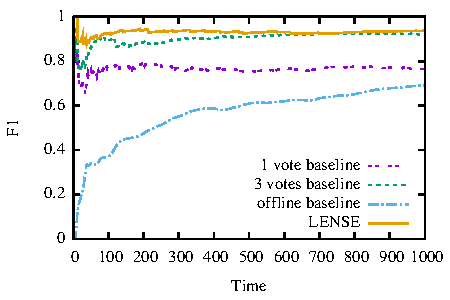
\includegraphics[width=1.0\textwidth]{figures/ner_2_class/f1_plot/f1_vs_time.pdf}
  \end{centering}
  \caption{A figure showing the comparative F1 vs time of several real-time regimes. The purple line is our system, costing just 0.65 queries per token. The green line is the 3-vote human baseline, costing 3 queries per token. The red line is the 1-vote baseline. The blue line is the performance of our classifier on its own, if we didn't allow it to query humans, and only gave it gold labels after classification in order to train.}
\label{fig:ner-running-f1}
\end{figure}

\paragraph{In the limit do we still need the crowd?}
We refer to \figureref{sentiment-tradeoff}.
We report results under two different sets of features for the sentiment task: \{unigrams, bigrams\}, and \{unigrams, bigrams, Socher et al recursive sentence embeddings\todo{cite}\}.
Given less model capacity, using only unigram and bigram features, our model soon saturates and must compensate for lack of represenational capacity with higher costs.
With richer embedding features, the model takes longer to learn, but eventually is able to reduce costs while maintaining accuracy preferences.
This suggests that given a sufficiently rich model, costs can be brought to zero in the limit.

\paragraph{Does LENSE exploit structure?}
First see \figureref{ner-cost}.
The jagged noise in the floating average of the cost plot is a sign that the system is taking advantage of the model to turn in {\em many classifications without human intervention}.
Behavioral analysis reveals the model is also taking advantage of the structure of queries to redistributed human effort to maximize accuracy.
As a representative example of this querying behavior from the evaluation set, take observed behavior when tagging the sentence:

\begin{center}
\textit{``U.S.\ says still committed to Cuba migration pacts.''}
\end{center}

The system, having never seen the token before, starts with a belief that Cuba is 59\% Person, 37\% Location, and 3\% None. The system knows already, from previously learned examples, that ``U.S.'' is a Location with 97\% probability. It immediately fires off two queries about ``Cuba,'' and waits 4 seconds for both responses to return Location. It now believes that ``Cuba'' is a Location with 95\% probability, and decides to turn in its current guess. This guess is added to the training set, and the model is updated.

\begin{figure}[t]
  \begin{centering}
  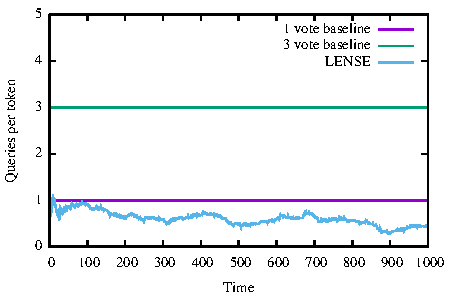
\includegraphics[width=1.0\textwidth]{figures/ner_2_class/cost_plot/cost_vs_time.pdf}
  \end{centering}
  \caption{A figure showing the number of queries required by our system, the 1 and 3 human query baselines over time.}
\label{fig:ner-cost}
\end{figure}

\paragraph{Are we learning a good model?}
We receive very noisy and sparse supervision.
Despite this, to reduce the costs in the future, our system must learn to generalize well.
We refer to \figureref{ner-dev-f1}.
We note that although our model is receiving supervisition signal at roughly 1/15 the rate of a fully observed online learning scenario\footnote{this calculation assumes ``fully observed'' is approximated by 3 human labels per example}, we track roughly parallel to the fully supervised line.

\begin{figure}[t]
  \begin{centering}
  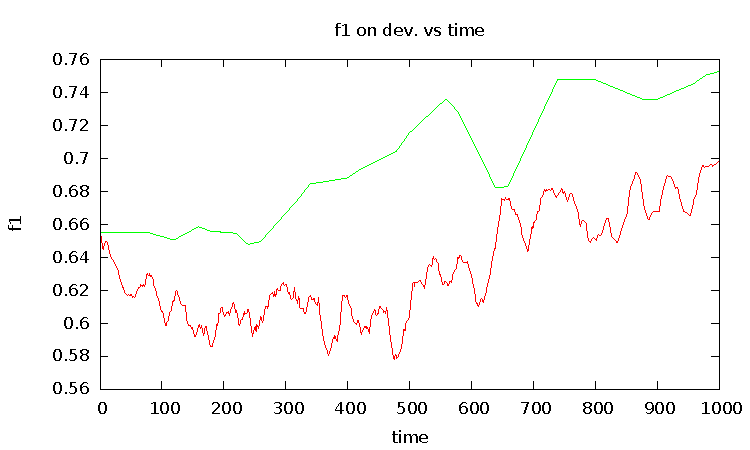
\includegraphics[width=1.0\textwidth]{figures/ner_2_class/machine_f1_plot/machine_f1_vs_time.pdf}
  \end{centering}
  \caption{A figure showing the relationship between the classifier we train, and one trained on gold labeled data. Evaluation is on a held out dev set. Note that our classifier learns more slowly because we are handing it a noisy approximation to train on, but the classifier narrows the gap as it gets more data.}
\label{fig:ner-dev-f1}
\end{figure}

\begin{figure}[t]
  \begin{centering}
  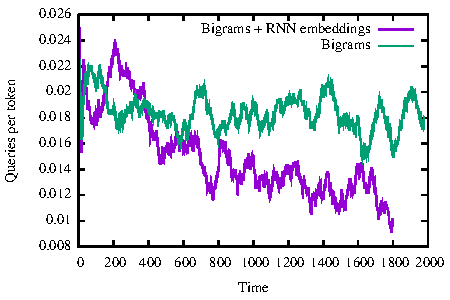
\includegraphics[width=1.0\textwidth]{figures/sentiment_cost_per_token_vs_time/cost_per_token_vs_time.pdf}
  \end{centering}
  \caption{A figure showing that increasing model capacity with richer distributional features (red line) enables the model to reduce costs further over time, compared with a simpler bag-of-words model with less representational capacity (green line).}
\label{fig:sentiment-tradeoff}
\end{figure}
